% Documento final del Proyecto Integrador 1.
% Compila con pdfLaTeX (Overleaf) o con XeLaTeX/Tectonic:  tectonic informe_final.tex
\documentclass[11pt,a4paper]{article}

\usepackage{iftex}
\ifPDFTeX
  \usepackage[utf8]{inputenc}
  \usepackage[T1]{fontenc}
  \usepackage{lmodern}
\else
  \usepackage{fontspec}
\fi
\usepackage[spanish,es-noshorthands,es-tabla]{babel}
\usepackage[margin=2.4cm]{geometry}
\usepackage{microtype}
\usepackage{graphicx}
\usepackage{booktabs}
\usepackage{tabularx}
\usepackage{array}
\usepackage{xcolor}
\usepackage{enumitem}
\usepackage{float}
\usepackage{caption}
\usepackage{pdflscape}
\usepackage{afterpage}
\usepackage{titlesec}
\usepackage{fancyhdr}
\usepackage[hidelinks]{hyperref}
\usepackage{xurl}

\definecolor{senal}{HTML}{B88A00}
\definecolor{asfalto}{HTML}{2E3136}
\definecolor{suave}{HTML}{6B7078}

\graphicspath{{figuras/}}
\setlength{\parskip}{0.45em}
\setlength{\parindent}{0pt}
\linespread{1.08}
\setlist{itemsep=0.25em, topsep=0.3em}
\captionsetup{font=small, labelfont={color=asfalto,bf}, margin=0.5cm}
\titleformat{\section}{\Large\bfseries\color{asfalto}}{\thesection.}{0.6em}{}
\titleformat{\subsection}{\large\bfseries\color{asfalto}}{\thesubsection}{0.6em}{}
\titleformat{\subsubsection}{\normalsize\bfseries\color{asfalto}}{\thesubsubsection}{0.6em}{}
\pagestyle{fancy}
\fancyhf{}
\fancyhead[L]{\small\color{suave}Gravedad de los siniestros viales en Colombia}
\fancyhead[R]{\small\color{suave}Proyecto Integrador 1}
\fancyfoot[C]{\small\thepage}
\renewcommand{\headrulewidth}{0.3pt}
\setlength{\headheight}{14pt}

\newcommand{\figura}[3]{%
  \begin{figure}[H]
    \centering
    \includegraphics[width=#2\textwidth]{#1}
    \caption{#3}
  \end{figure}}

\begin{document}

% ------------------------------------------------------------------ portada
\hypersetup{pageanchor=false}
\begin{titlepage}
  \thispagestyle{empty}
  {\color{senal}\rule{\textwidth}{2pt}}
  \vspace{2.2cm}

  {\small\color{suave}MAESTRÍA EN CIENCIA DE DATOS Y ANALÍTICA \\ PROYECTO INTEGRADOR 1 · DOCUMENTO FINAL}

  \vspace{0.8cm}
  {\fontsize{26}{31}\selectfont\bfseries\color{asfalto}\raggedright\hyphenpenalty=10000\exhyphenpenalty=10000
  Predicción de la gravedad de los siniestros viales en Colombia a partir del vehículo involucrado\par}

  \vspace{0.6cm}
  {\large\color{suave}Un flujo de datos en AWS, un modelo calibrado y un tablero para las autoridades de tránsito, construidos sobre el registro público del RUNT\par}

  \vspace{2cm}
  {\large\bfseries\color{asfalto}Integrantes\par}
  \vspace{0.3cm}
  \begin{tabular}{@{}l@{}}
    Santiago Acevedo Urrego \\
    Daniel Felipe Arango Guarín \\
    Santiago Betancur \\
    Daniel Correa Botero \\
    Miguel Ángel Cano Salinas
  \end{tabular}

  \vfill
  \begin{tabularx}{\textwidth}{@{}lX@{}}
    \color{suave}Materias & SI7009 Aprendizaje Automático · SI7006 Almacenamiento y Procesamiento de Grandes Datos · SI7007 Visualización de Datos \\[0.3em]
    \color{suave}Fecha & Noviembre de 2026 \\[0.3em]
    \color{suave}Repositorio & \url{https://github.com/stufonn-cell/accidentes_project_for_data_science} \\[0.3em]
    \color{suave}Datos & Ministerio de Transporte, RUNT. Vehículos involucrados en un accidente de tránsito, Ley 2251 de 2022. datos.gov.co, licencia CC BY-SA 4.0
  \end{tabularx}
  \vspace{0.5cm}
  {\color{senal}\rule{\textwidth}{2pt}}
\end{titlepage}
\hypersetup{pageanchor=true}

\setcounter{tocdepth}{2}
\tableofcontents
\newpage

% ------------------------------------------------------------------ 1
\section{Introducción}

En Colombia, los siniestros viales siguen siendo una de las principales causas de muerte evitable. En 2024 murieron 8.271 personas en las vías del país, según cifras preliminares del Observatorio Nacional de Seguridad Vial (Vargas, 2025). Desde 2022, la Ley 2251, conocida como Ley Julián Esteban, obliga al RUNT a publicar los vehículos involucrados en siniestros con muertos o heridos. Ese registro ya es público para todo el país, pero no encontramos un análisis que diga qué perfiles de vehículo y qué contextos se asocian con los siniestros más graves.

Este documento reúne todas las entregas del Proyecto Integrador 1. Usamos el registro del RUNT para responder una pregunta concreta: a partir del vehículo y del contexto en que se registró el siniestro, ¿podemos anticipar cuáles siniestros con víctimas tienen más riesgo de terminar con muertos, con un modelo que también funcione en municipios que no vio al entrenar?

El proyecto tiene cuatro piezas que se conectan entre sí:

\begin{itemize}
  \item Un flujo de datos en AWS que descarga el registro, lo valida, lo limpia y deja tablas listas para analizar, organizado como un lago de datos por zonas.
  \item Un análisis exploratorio que encontró problemas serios de cobertura en el registro y los corrigió antes de entrenar.
  \item Un modelo de clasificación que entrega una probabilidad calibrada, publicado como servicio web, y un agrupamiento de municipios que ayuda a evaluarlo.
  \item Un tablero web pensado para las autoridades de tránsito, que cuenta los hallazgos en orden y deja explorar los datos con filtros.
\end{itemize}

Uno de los resultados más importantes apareció antes del modelo. El registro tiene huecos grandes: Medellín y Bogotá casi dejaron de reportar en 2025, y Medellín subió en un solo mes más de veinte mil reportes atrasados. Si esos problemas no se tratan, cambian las conclusiones. Por eso dedicamos una parte importante del trabajo a entender y corregir la calidad del dato, y lo contamos con detalle.

El documento sigue el orden sugerido para la entrega. La sección~\ref{sec:marco} presenta el marco teórico. La sección~\ref{sec:metodo} recorre el desarrollo del modelo, desde el problema hasta la evaluación y su utilidad. La sección~\ref{sec:tecnologia} describe la ingeniería de datos y la arquitectura en AWS. La sección~\ref{sec:visualizacion} explica cómo diseñamos y validamos el tablero. Al final están las conclusiones generales y las referencias.

% ------------------------------------------------------------------ 2
\section{Marco teórico}\label{sec:marco}

\subsection{La seguridad vial como problema de salud pública}

La Organización Mundial de la Salud estima 1,19 millones de muertes al año en las vías. Son la primera causa de muerte entre los 5 y los 29 años, y más de la mitad de los fallecidos son peatones, ciclistas y motociclistas, sobre todo en países de ingresos bajos y medios (OMS, 2023). Colombia sigue ese patrón: entre enero y abril de 2025 murieron 2.529 personas en las vías, y cerca del 62~\% eran motociclistas (Agencia Nacional de Seguridad Vial, 2025). En nuestros datos, las motocicletas son el 56,7~\% de los vehículos involucrados.

La respuesta del Estado se apoya en el enfoque de sistema seguro. Este enfoque parte de que las personas cometen errores y de que el sistema vial debe diseñarse para que esos errores no terminen en muertes, actuando sobre las vías, las velocidades, los vehículos y los usuarios. La Ley 2251 de 2022 ordena formular la política de seguridad vial con este enfoque (Congreso de la República, 2022), y el Plan Nacional de Seguridad Vial 2022-2031 lo toma como guía e incluye la gestión del conocimiento entre sus líneas de acción (Ministerio de Transporte, 2022). El artículo 11 de esa ley es el que obliga al RUNT a publicar el registro que usamos (Ministerio de Transporte, 2026).

\subsection{Modelos para la gravedad de los siniestros}

Los estudios de gravedad de siniestros pasaron de modelos logit y probit al aprendizaje automático, que capta relaciones no lineales e interacciones entre variables (Savolainen et al., 2011; Mannering y Bhat, 2014). Los árboles de decisión parten los datos con reglas simples. Los bosques aleatorios combinan muchos árboles entrenados sobre muestras distintas (Breiman, 2001), y Extra Trees hace lo mismo con cortes más aleatorios (Geurts et al., 2006). El gradient boosting construye árboles pequeños en secuencia, y cada uno corrige los errores de los anteriores (Friedman, 2001); XGBoost y LightGBM lo hicieron eficiente en tablas grandes (Chen y Guestrin, 2016; Ke et al., 2017). La regresión logística sigue siendo la referencia lineal: es simple y fácil de interpretar.

\subsection{Evaluar cuando el evento es raro}

Cuando los casos positivos son pocos, la exactitud engaña: un modelo que nunca alerta acierta casi siempre. La curva de precisión y sensibilidad describe mejor el desempeño en la clase minoritaria que la curva ROC (Saito y Rehmsmeier, 2015), y su área, la PR-AUC, tiene como referencia la proporción de positivos. Los pesos por clase y el ajuste del umbral ayudan con el desbalance (He y Garcia, 2009). Si las probabilidades están calibradas, el umbral que minimiza el costo esperado se calcula directamente a partir de lo que cuesta cada tipo de error (Elkan, 2001). La regresión isotónica es una forma sencilla de calibrar (Zadrozny y Elkan, 2002).

Cuando las filas no son independientes, la validación cruzada común filtra información. En este proyecto varios vehículos pueden pertenecer al mismo siniestro, y cada siniestro ocurre en un solo municipio y un solo mes. Por eso validamos por grupos de municipios y por periodos, para que los datos de prueba nunca aparezcan en el entrenamiento.

\subsection{Agrupamiento}

K-means agrupa las observaciones según su cercanía al centro de cada grupo (MacQueen, 1967), y el agrupamiento jerárquico de Ward une grupos minimizando la varianza interna. El número de grupos se puede elegir con el coeficiente de silueta, que compara qué tan cerca está cada punto de su grupo frente al grupo vecino (Rousseeuw, 1987).

\subsection{Lagos de datos y comunicación visual}

Un lago de datos guarda la información en almacenamiento de objetos, organizada por zonas que van de lo crudo a lo listo para analizar. La versión más difundida usa tres capas, bronce, plata y oro, y guarda las tablas en formatos columnares que un motor SQL consulta directamente (Armbrust et al., 2021). Para la visualización seguimos el marco de Munzner (2014), que pide definir qué datos se muestran, por qué tarea los necesita el usuario y cómo se codifican, y las recomendaciones de Knaflic (2015) sobre títulos que cuentan el hallazgo y el uso del color solo para resaltar lo importante.

\subsection{Metodología}

Seguimos CRISP-DM (Chapman et al., 2000), que organiza el trabajo en seis fases que se repiten en ciclos: entendimiento del negocio, entendimiento de los datos, preparación, modelado, evaluación y despliegue. El ciclo se notó en la práctica: lo que encontramos al evaluar los primeros modelos nos llevó a volver a preparar los datos, por ejemplo para corregir la edad del vehículo y repartir las cargas masivas.

% ------------------------------------------------------------------ 3
\section{Desarrollo metodológico del modelo}\label{sec:metodo}

\subsection{Entendimiento del problema}

\textit{Decisión que apoya.} Las secretarías de movilidad, la Agencia Nacional de Seguridad Vial y la policía de tránsito tienen recursos limitados para controles, campañas y revisiones. El modelo les ayuda a decidir hacia qué perfiles de vehículo y qué contextos dirigirlos, y a detectar municipios cuya letalidad se aleja mucho de lo esperado.

\textit{Tarea de aprendizaje automático.} Es una clasificación binaria supervisada con salida de probabilidad. Cada fila es un vehículo involucrado en un siniestro con víctimas. La variable objetivo vale 1 si el siniestro fue con muertos y 0 si fue solo con heridos. Las variables de entrada describen el vehículo, que son el tipo, la marca, el año del modelo y la edad, y el contexto del registro, que son el mes, el departamento y la autoridad de tránsito.

\textit{Hipótesis.} Planteamos tres:

\begin{enumerate}
  \item El tipo de vehículo y el tipo de vía se asocian con la gravedad. Esperábamos que los vehículos de carga y los siniestros en carretera fueran más letales.
  \item El vehículo por sí solo explica poco. Esperábamos que el contexto pesara más que la marca o la edad.
  \item Una parte de las diferencias entre municipios es forma de reportar y no riesgo real.
\end{enumerate}

\textit{Supuestos y restricciones.} La gravedad es del siniestro y no del vehículo: si chocan un camión y una moto y muere el motociclista, los dos quedan con muertos. Por eso el modelo encuentra asociaciones y no dice qué vehículo causó la muerte. La fuente no trae día, hora, dirección, causa ni datos de las víctimas, y solo incluye siniestros con víctimas. El municipio no entra como variable, porque el modelo debe servir en municipios que no vio.

\textit{Criterios de éxito.} Una PR-AUC claramente por encima de la proporción de casos con muertos, que es 0,053; probabilidades calibradas, que se puedan leer como frecuencias; y un desempeño que se mantenga entre grupos de municipios.

\subsection{Análisis exploratorio de datos}

\subsubsection{Entendimiento de los datos}

Usamos una sola fuente: el conjunto «Vehículos involucrados en un accidente de tránsito, Ley 2251 de 2022», que publica el Ministerio de Transporte con datos del RUNT (Ministerio de Transporte, 2026). Es un CSV de unos 50 MB con 450.335 filas y 9 columnas, de enero de 2022 a septiembre de 2026, que cubre 689 municipios de 31 departamentos. No tiene datos personales. La tabla~\ref{tab:variables} resume las variables.

\begin{table}[H]
\centering\small
\caption{Variables de la fuente.}\label{tab:variables}
\begin{tabularx}{\textwidth}{@{}lrX@{}}
\toprule
Variable & Valores & Lo que encontramos \\
\midrule
TIPO\_VEHICULO & 31 & Motocicletas 56,7~\%, automóviles 22,2~\%, camionetas 8,5~\%, buses 3,9~\%, camiones 2,7~\% \\
MARCA\_VEHICULO & 381 & 64 marcas tienen 200 filas o más; el resto son marcas pequeñas \\
MODELO\_VEHICULO & 88 & Año del modelo, de 1937 a 2027; 83 valores son imposibles \\
EDAD\_VEHICULO & 90 & 20 vacíos, dos valores mal escritos y una edad calculada a la fecha de publicación, no del siniestro \\
FECHA\_ACCIDENTE & 57 & Solo mes y año, de 01/2022 a 09/2026 \\
GRAVEDAD\_ACCIDENTE & 2 & Con heridos o con muertos: es la variable objetivo \\
DEPARTAMENTO\_ACCIDENTE & 31 & \\
MUNICIPIO\_ACCIDENTE & 663 & 689 municipios al combinar el nombre con el departamento \\
AUTORIDAD\_DE\_TRANSITO & 237 & La policía de carreteras aparece en 645 municipios \\
\bottomrule
\end{tabularx}
\end{table}

\textit{El evento es raro.} Hay 23.899 registros con muertos de 450.335, el 5,3~\%. Un modelo que siempre diga «con heridos» acertaría el 94,7~\% de las veces sin servir para nada. Además, 202 municipios no tienen ningún registro con muertos y 261 tienen diez o más.

\textit{Cada fila es un vehículo y no un siniestro.} No hay un identificador del siniestro, así que no se sabe qué vehículos chocaron entre sí. 159.399 filas son idénticas a otra en las nueve columnas. No las quitamos: dos motos de la misma marca y modelo en el mismo municipio y mes producen la misma fila, y borrarlas eliminaría vehículos reales. Para distinguirlas, el flujo le asigna a cada fila un identificador propio, de RUNT-000001 a RUNT-450335.

\textit{La cobertura cambia mucho en el tiempo.} Esta fue la sorpresa más grande. Medellín pasa de 27.821 registros en 2024 a 201 en 2025, y Bogotá de 19.184 a 4.526, mientras el resto del país sube un 8~\%. Además, en julio de 2024 Medellín publicó 22.667 registros en un solo mes, 8,8 veces su mes normal, y solo el 0,04~\% con muertos. Son reportes atrasados que entraron todos con la misma fecha. La figura~\ref{fig:caida} muestra la caída y la figura~\ref{fig:medellin} la carga masiva.

\figura{cal_volumen}{0.82}{Vehículos reportados en 2024 y 2025. Medellín y Bogotá casi dejan de reportar; el resto del país sube. Fuente: tablero del proyecto.\label{fig:caida}}

\figura{cal_medellin}{0.82}{Reportes de Medellín por mes. La barra amarilla de julio de 2024 son reportes atrasados que entraron con esa fecha; después de noviembre de 2024 la ciudad casi no reporta.\label{fig:medellin}}

\subsubsection{Preparación de los datos}

Cada problema que encontramos se convirtió en una decisión dentro del flujo de datos. La tabla~\ref{tab:decisiones} las resume. Todas quedan en código, en la capa silver, y se repiten igual cada vez que corre el flujo.

\begin{table}[H]
\centering\small
\caption{Hallazgos del análisis exploratorio y decisiones de preparación.}\label{tab:decisiones}
\begin{tabularx}{\textwidth}{@{}>{\raggedright\arraybackslash}X>{\raggedright\arraybackslash}X@{}}
\toprule
Hallazgo & Decisión \\
\midrule
La edad de la fuente se calculó a la fecha de publicación: sobra 5 años en 2022 y 1 en 2026 & Se recalcula como año del siniestro menos año del modelo, con mínimo 0 \\
381 marcas, muchas con pocas filas & Las marcas con menos de 200 filas se agrupan como OTRAS \\
31 tipos, 20 con menos de mil filas & Los tipos con menos de mil filas se agrupan como OTRO \\
237 autoridades, muchas pequeñas & El modelo agrupa las que tienen menos de 100 filas \\
83 años de modelo imposibles & Se marcan y quedan sin edad; no se borran \\
Textos con y sin tildes, como SECRETARÍA y SECRETARIA & Se quitan tildes y espacios y se pasa a mayúsculas \\
Nombres de municipio repetidos en varios departamentos & La clave es el municipio junto con su departamento \\
64 cargas masivas en 31 municipios & El mes conserva su número normal de registros y el exceso se reparte entre los meses anteriores del mismo municipio \\
Meses con caídas o que siguen anómalos & Esas filas y las reubicadas no entran al entrenamiento \\
\bottomrule
\end{tabularx}
\end{table}

\textit{Cómo se reparten las cargas masivas.} Para cada municipio comparamos el número de registros de cada mes con su mediana mensual de 2022 a 2024. Un mes con más de tres veces esa mediana es una carga masiva, y uno con menos del 20~\% es una caída. Solo juzgamos los 129 municipios que reportan al menos cinco registros al mes, porque en los pequeños las variaciones son azar. Cuando hay una carga masiva, el mes se queda con su mediana, elegida al azar con una semilla fija, y el resto de los registros pasa a los meses anteriores en proporción a lo que reportó cada uno. Así se conserva la forma de la serie. Un vehículo nunca se mueve a un año anterior al de su modelo menos uno. En total se reubicaron 21.230 registros, casi todos de Medellín: de los 22.667 de julio de 2024, ese mes conserva 2.589 y los otros 20.078 se reparten entre enero de 2022 y junio de 2024. Cada fila movida guarda el mes en que se publicó, para poder deshacer el cambio.

\textit{Qué se deja fuera del entrenamiento.} Los 21.230 registros reubicados y otros 2.522 que caen en meses que siguen anómalos después del reparto, 23.752 en total, el 5,3~\% de los datos. Los años 2025 y 2026, con la cobertura cambiada, se evalúan aparte. La figura~\ref{fig:tratamiento} resume este tratamiento tal como lo muestra el tablero.

\figura{fig_tratamiento}{1}{Decisiones de preparación y etapas del flujo, tal como aparecen en la página 4 del tablero.\label{fig:tratamiento}}

\subsubsection{Análisis descriptivo y hallazgos}

Con los datos ya limpios, de cada 100 vehículos en siniestros con víctimas, 5,5 estuvieron en uno con muertos. Los hallazgos principales son estos:

\begin{itemize}
  \item \textit{Los vehículos de carga son los más letales.} El tractocamión llega a 28,7~\%, 5,2 veces el promedio, seguido de la volqueta y el camión, como muestra la figura~\ref{fig:tipo}. Los automóviles quedan en 2,8~\%.
  \item \textit{Las motos concentran los casos.} Su letalidad está cerca del promedio, pero son tantas que aportan el 54~\% de los casos mortales: 12.717 vehículos.
  \item \textit{La edad pesa poco hasta los 15 años.} La letalidad se mantiene entre 4,8~\% y 5,0~\% hasta los 10 años y sube a 9,2~\% en los vehículos de 21 años o más, como muestra la figura~\ref{fig:edad}.
  \item \textit{Quién registra importa mucho.} Los registros de la policía de carreteras tienen 22,3~\% de casos con muertos y los de las secretarías municipales 3,2~\%. En carretera hay más velocidad y los siniestros son más graves, pero también cada secretaría reporta distinto: Medellín tiene solo 0,6~\% de registros con muertos.
  \item \textit{Cesar es el departamento más letal}, con 33~\%, seguido de Magdalena, Caquetá y Cauca. Son departamentos donde una gran parte de los registros viene de la policía de carreteras.
\end{itemize}

\figura{per_tipo}{0.82}{Letalidad por tipo de vehículo. La línea marca el promedio de 5,5~\%.\label{fig:tipo}}

\figura{per_edad}{0.82}{Letalidad por edad del vehículo al momento del siniestro.\label{fig:edad}}

\textit{Correlación no es causa, y la composición engaña.} La proporción nacional de registros con muertos sube de 5,1~\% en 2024 a 7,4~\% en 2025. Parece que las vías se volvieron más peligrosas, pero al quitar Medellín y Bogotá la proporción es 7,7~\% en los dos años, como muestra la figura~\ref{fig:composicion}. El salto se explica porque dejaron de reportar las dos ciudades que más siniestros con heridos registraban. Es un cambio en quién reporta, no en el riesgo. Este hallazgo nos llevó a evaluar 2025 y 2026 aparte.

\figura{cal_letalidad}{0.82}{Letalidad nacional con y sin Medellín y Bogotá. Sin esas dos ciudades no hay salto.\label{fig:composicion}}

\subsection{Selección de modelos, características, entrenamiento y evaluación}

\subsubsection{Modelos}

Comparamos cinco clasificadores contra una referencia sin modelo:

\begin{itemize}
  \item La referencia asigna a todos la misma probabilidad, la proporción de casos con muertos. Es el piso que cualquier modelo debe superar.
  \item Regresión logística, como modelo lineal de base.
  \item Árbol de decisión.
  \item Tres ensambles de árboles: bosque aleatorio, Extra Trees y gradient boosting, en su versión por histogramas de scikit-learn.
\end{itemize}

Para la parte no supervisada comparamos k-means con el agrupamiento jerárquico de Ward sobre los municipios.

\subsubsection{Características e ingeniería de características}

El modelo usa siete variables. Del vehículo: el tipo agrupado, la marca agrupada, el año del modelo y la edad recalculada al momento del siniestro. Del contexto: el mes, el departamento y la autoridad de tránsito. Las variables nuevas salen directamente de los hallazgos del análisis exploratorio, como muestra la tabla~\ref{tab:decisiones}.

El municipio no es variable. El modelo se piensa para municipios que no vio, y la validación deja siempre el municipio de prueba fuera del entrenamiento, así que un identificador de municipio solo inflaría el ajuste. La autoridad sí entra: la policía de carreteras está en 645 municipios y su información se transfiere a municipios nuevos.

Toda la preparación para el modelo, es decir la codificación de categorías, el reemplazo de vacíos y el escalado, va dentro de un pipeline de scikit-learn que se ajusta solo con los datos de entrenamiento de cada partición. Así no hay fuga de información por preparar los datos antes de dividirlos.

\subsubsection{Entrenamiento}

Entrenamos con 2022, 2023 y 2024, sin los meses anómalos ni las filas reubicadas: 327.068 filas, con 4,8~\% de casos con muertos. El proceso tiene tres pasos:

\begin{enumerate}
  \item \textit{Búsqueda de hiperparámetros.} Una búsqueda en rejilla con validación cruzada agrupada por municipio en cinco particiones, usando la PR-AUC como puntaje, sobre una muestra de 120.000 filas para que el flujo corra en pocos minutos. Para la regresión logística probamos tres niveles de regularización y ganó el más fuerte. Para el gradient boosting probamos 12 combinaciones de tasa de aprendizaje, tamaño de árbol y regularización; ganó una tasa de 0,1 con árboles de 31 hojas y regularización. Los demás árboles usan configuraciones fijas para no multiplicar el tiempo. La propuesta inicial planeaba usar optuna; como AWS Glue solo trae scikit-learn, usamos una rejilla pequeña y sistemática.
  \item \textit{Selección.} Comparamos los cinco modelos con la misma validación agrupada por municipio sobre las 327.068 filas. Los municipios de validación nunca se ven al entrenar, y como cada siniestro ocurre en un solo municipio, sus vehículos no quedan repartidos entre entrenamiento y prueba. Se elige el de mayor PR-AUC promedio.
  \item \textit{Prueba temporal.} Con el conjunto de prueba intacto hasta el final, entrenamos con 2022 y 2023, 226.539 filas, y probamos con 2024, 100.529 filas. Cada modelo se calibra con regresión isotónica.
\end{enumerate}

Todos los modelos usan pesos por clase para compensar el desbalance. No probamos la submuestra de la clase mayoritaria que mencionaba la propuesta.

\subsubsection{Evaluación}

\textit{Métrica principal.} Usamos la PR-AUC porque mide qué tan bien quedan los casos con muertos arriba en la lista, que es justo lo que necesita quien prioriza. Su valor de referencia es la proporción de positivos: 0,052 en 2024. La ROC-AUC se ve bien aunque haya muchas falsas alarmas, porque los casos sin muertos son muchísimos; la reportamos como complemento.

\textit{Resultados.} La tabla~\ref{tab:resultados} muestra la prueba con 2024. El gradient boosting gana la selección por municipio y también tiene la mejor PR-AUC, ROC-AUC y F1 en 2024. El árbol de decisión queda casi empatado en PR-AUC.

\begin{table}[H]
\centering\small
\caption{Prueba temporal: entrenamiento con 2022 y 2023, prueba con 2024.}\label{tab:resultados}
\begin{tabular}{@{}lcccccc@{}}
\toprule
Modelo & PR-AUC & ROC-AUC & Precisión & Sensibilidad & F1 & Exactitud bal. \\
\midrule
Referencia sin modelo & 0,052 & 0,500 & -- & -- & -- & 0,500 \\
Regresión logística & 0,221 & 0,825 & 0,199 & 0,612 & 0,300 & 0,739 \\
Bosque aleatorio & 0,215 & 0,817 & 0,203 & 0,572 & 0,299 & 0,724 \\
Extra Trees & 0,207 & 0,814 & 0,195 & 0,567 & 0,291 & 0,719 \\
Árbol de decisión & 0,232 & 0,816 & 0,200 & 0,610 & 0,302 & 0,738 \\
Gradient boosting & 0,232 & 0,825 & 0,206 & 0,607 & 0,308 & 0,739 \\
\bottomrule
\end{tabular}
\end{table}

La PR-AUC del gradient boosting en 2024 es 0,232, 4,5 veces la referencia. Supera la meta, pero el valor absoluto es modesto: la señal del vehículo es débil, como anticipaba la segunda hipótesis. La figura~\ref{fig:prauc} muestra la comparación tal como aparece en el tablero.

\figura{mod_prauc}{0.75}{PR-AUC de cada modelo en la prueba de 2024.\label{fig:prauc}}

\textit{La validación por municipio es más dura que la temporal.} En 2024 el modelo ya conoce las autoridades de cada municipio y logra 0,232. En municipios nuevos baja a 0,162 en promedio, 3,1 veces la referencia, y varía mucho entre particiones: 0,034; 0,122; 0,231; 0,211 y 0,214. La de 0,034 es Medellín sola, con apenas 0,65~\% de casos con muertos, porque reporta muchos siniestros con heridos y muy pocos con muertos.

\textit{Calibración.} Los pesos por clase inflan las probabilidades. Sin calibrar, el error de Brier del gradient boosting en 2024 es 0,170, peor que predecir siempre la proporción de positivos, que da 0,049. Con la calibración isotónica baja a 0,044, y las probabilidades coinciden con lo observado: en el décimo de registros con más riesgo, el modelo predice en promedio 24,2~\% y la tasa real es 24,5~\%. Gracias a esto las probabilidades se pueden leer como frecuencias.

\textit{Sesgo y varianza.} En la validación por municipio, el gradient boosting tiene una PR-AUC de 0,259 en entrenamiento y 0,162 en validación. Con la curva de aprendizaje, al pasar de 8.677 a 86.776 filas, la PR-AUC de entrenamiento baja de 0,298 a 0,255 y la de validación sube de 0,133 a 0,158. La brecha se cierra y las dos curvas quedan bajas: domina el sesgo, es decir, faltan variables más que datos. Más filas del mismo tipo ayudarían poco; harían falta el tipo de vía, la hora o el número de víctimas, que el registro no trae.

\textit{Errores por segmento.} Dentro de cada grupo de municipios la ROC-AUC baja: 0,58 en los municipios de carretera y 0,66 en los urbanos, frente a 0,71 en total. Buena parte de lo que el modelo sabe es distinguir la ciudad de la carretera; dentro de un mismo tipo de municipio discrimina poco.

\textit{Qué variables pesan.} Medimos cuánto cae la PR-AUC al desordenar cada variable. La autoridad de tránsito es la que más pesa, con una caída de 0,153, seguida del departamento con 0,031 y el tipo de vehículo con 0,018. La marca, la edad, el modelo y el mes casi no suman una vez se conocen el tipo y el contexto. La figura~\ref{fig:importancia} lo muestra.

\figura{mod_importancia}{0.75}{Importancia de cada variable, medida como la caída de la PR-AUC al desordenarla.\label{fig:importancia}}

\subsection{Análisis y conclusiones del modelo}

\textit{Del desempeño al impacto.} Supusimos que dejar pasar un siniestro con muertos cuesta diez veces más que una falsa alarma, por ejemplo una inspección o una campaña mal dirigida. Con probabilidades calibradas, el umbral que minimiza el costo es 1 dividido entre 11, es decir 0,091. Lo comprobamos en 2024: el mejor umbral de una rejilla de 0,02 a 0,49 fue 0,09, prácticamente el mismo.

La tabla~\ref{tab:negocio} compara el modelo con las alternativas que hoy tiene una autoridad de tránsito.

\begin{table}[H]
\centering\small
\caption{Estrategias en 2024: 100.529 registros, 5.227 con muertos.}\label{tab:negocio}
\begin{tabularx}{\textwidth}{@{}Xcccc@{}}
\toprule
Estrategia & Revisados & Casos hallados & Precisión & Costo por registro \\
\midrule
No alertar nada & 0~\% & 0~\% & -- & 0,520 \\
Alertar todo & 100~\% & 100~\% & 5,2~\% & 0,948 \\
Alertar al azar & 15,3~\% & 15,3~\% & 5,2~\% & -- \\
Regla simple: carga o policía de carreteras & 12,8~\% & 51,4~\% & 20,8~\% & 0,354 \\
Modelo con umbral 0,091 & 15,3~\% & 60,6~\% & 20,6~\% & 0,326 \\
\bottomrule
\end{tabularx}
\end{table}

Con el modelo, revisar el 15~\% de los registros encuentra el 61~\% de los casos con muertos, 3.170 de 5.227, cuatro veces lo que daría escoger al azar. Frente a no hacer nada, el costo baja 37~\%. Frente a la regla simple, que ya captura lo más obvio, baja 8~\%. Dicho de otra forma, la regla simple se lleva buena parte del valor y el modelo agrega una mejora moderada, sobre todo porque ordena los casos con probabilidades útiles en lugar de un sí o un no.

\figura{fig_utilidad}{0.9}{Casos con muertos que encuentra cada estrategia en 2024 con un esfuerzo de revisión parecido.\label{fig:utilidad}}

\textit{Letalidad observada frente a esperada.} Para cada municipio comparamos la proporción real de casos con muertos con la que predice un modelo que nunca lo vio. Medellín tiene 0,5~\% frente a 3,3~\% esperado, una razón de 0,16. Lo más probable es que haya subregistro de muertos o sobrerregistro de heridos, no que la ciudad sea seis veces más segura. El patrón se repite en Girardota, Urrao y Sabaneta. En el otro extremo, Soacha tiene 15,7~\% frente a 4,2~\% esperado, y Yopal, Floridablanca y Bogotá también superan con claridad lo esperado. Estos municipios son alertas para revisar, primero la calidad del registro y luego el riesgo real.

\textit{Caso aplicado.} La tabla~\ref{tab:casos} muestra el modelo final sobre perfiles concretos.

\begin{table}[H]
\centering\small
\caption{Probabilidad de que el siniestro sea con muertos para cinco perfiles.}\label{tab:casos}
\begin{tabularx}{\textwidth}{@{}Xcc@{}}
\toprule
Perfil & Probabilidad & ¿Alerta? \\
\midrule
Tractocamión Kenworth 2012 en el Cesar, policía de carreteras, diciembre & 0,424 & Sí \\
Moto AKT 2023 en Antioquia, policía de carreteras, junio & 0,185 & Sí \\
Bus Chevrolet 2010 en Boyacá, policía de carreteras, enero & 0,181 & Sí \\
Automóvil Chevrolet 2015, secretaría de Bogotá, marzo & 0,019 & No \\
La misma moto AKT 2023, secretaría de Medellín, junio & 0,005 & No \\
\bottomrule
\end{tabularx}
\end{table}

El tractocamión en carretera es el perfil de más riesgo: 0,42 es ocho veces la proporción general, y coincide con lo que mostró el análisis exploratorio. La misma moto pasa de 0,005 a 0,185 solo por cambiar la autoridad que registra. Ahí se ven el mayor acierto y el mayor riesgo del modelo: acierta en que un siniestro en carretera es más grave, pero parte de esa diferencia es que Medellín casi no registra siniestros con muertos. Una secretaría lo usaría para ordenar perfiles y elegir dónde poner controles, por ejemplo vehículos de carga y buses en corredores viales, y para revisar los municipios cuya letalidad se aleja mucho de lo esperado.

\textit{Agrupamiento de municipios.} Agrupamos los 210 municipios con 100 registros o más, que reúnen el 98,5~\% de los datos, según su letalidad, la edad promedio de los vehículos, la proporción de motos, de vehículos de carga y de registros de la policía de carreteras, y su volumen. K-means y Ward eligen dos grupos, con siluetas de 0,31 y 0,32. Dejamos k-means, como planteaba la propuesta. Los grupos son claros en su interpretación:

\begin{itemize}
  \item 97 municipios de carretera, con 28.156 registros, 24~\% de casos con muertos en promedio y 70~\% de registros de la policía de carreteras.
  \item 113 municipios urbanos, con 415.519 registros, 8~\% de casos con muertos y 62~\% de motos.
\end{itemize}

Las siluetas son bajas y los dos métodos coinciden poco, con un índice de Rand ajustado de 0,28. Los grupos son más un gradiente entre ciudad y carretera que tipos separados. Aun así sirvieron para ver que el modelo discrimina poco dentro de cada grupo.

\textit{Límites y riesgos.} El modelo aprende la forma de reportar de cada autoridad, no solo el riesgo, y no puede separar las dos cosas. En 2025 y 2026, con la cobertura cambiada, la PR-AUC es 0,271, pero la proporción de casos con muertos sube a 7,8~\% y el modelo alerta el 27~\% de los registros: la mezcla de quién reporta cambió y la calibración ya no es la de 2024. Antes de usarlo en un periodo nuevo hay que recalibrarlo.

\textit{Respuesta a las hipótesis.} La primera se confirma: los vehículos de carga y los siniestros en carretera son los más letales. La segunda también: el vehículo aporta poco frente al contexto. La tercera tiene evidencia fuerte: Medellín, la caída de 2025 y la importancia de la autoridad muestran que una parte de las diferencias es forma de reportar.

% ------------------------------------------------------------------ 4
\section{Tecnología: ingeniería de datos}\label{sec:tecnologia}

\subsection{Arquitectura de referencia}

Adoptamos un lago de datos por zonas con procesamiento por lotes. Los datos pasan por cuatro zonas en Amazon S3: raw guarda el CSV tal como llega, bronze lo guarda como texto con su identificador, silver lo deja limpio y con marcas de calidad, y gold tiene las tablas listas para el modelo, el tablero y las consultas.

Elegimos esta arquitectura por las características de la fuente:

\begin{itemize}
  \item \textit{Volumen.} Unos 50 MB y 450 mil filas. No hace falta un clúster permanente; basta con trabajos que se encienden, corren y se apagan.
  \item \textit{Velocidad.} El RUNT publica el archivo por lotes, unas pocas veces al año. No hay un flujo continuo de eventos, así que una arquitectura de streaming, como Kappa, o una con capa de velocidad, como Lambda, agregaría costo sin beneficio.
  \item \textit{Latencia.} El entrenamiento puede tardar minutos. Lo único que necesita responder rápido es la consulta al modelo, y para eso está la API.
\end{itemize}

Las zonas permiten volver atrás: si cambia una regla de limpieza, se recalcula desde raw sin volver a descargar nada. La figura~\ref{fig:arquitectura} muestra la arquitectura completa con los servicios de AWS.

\afterpage{%
\begin{landscape}
  \centering
  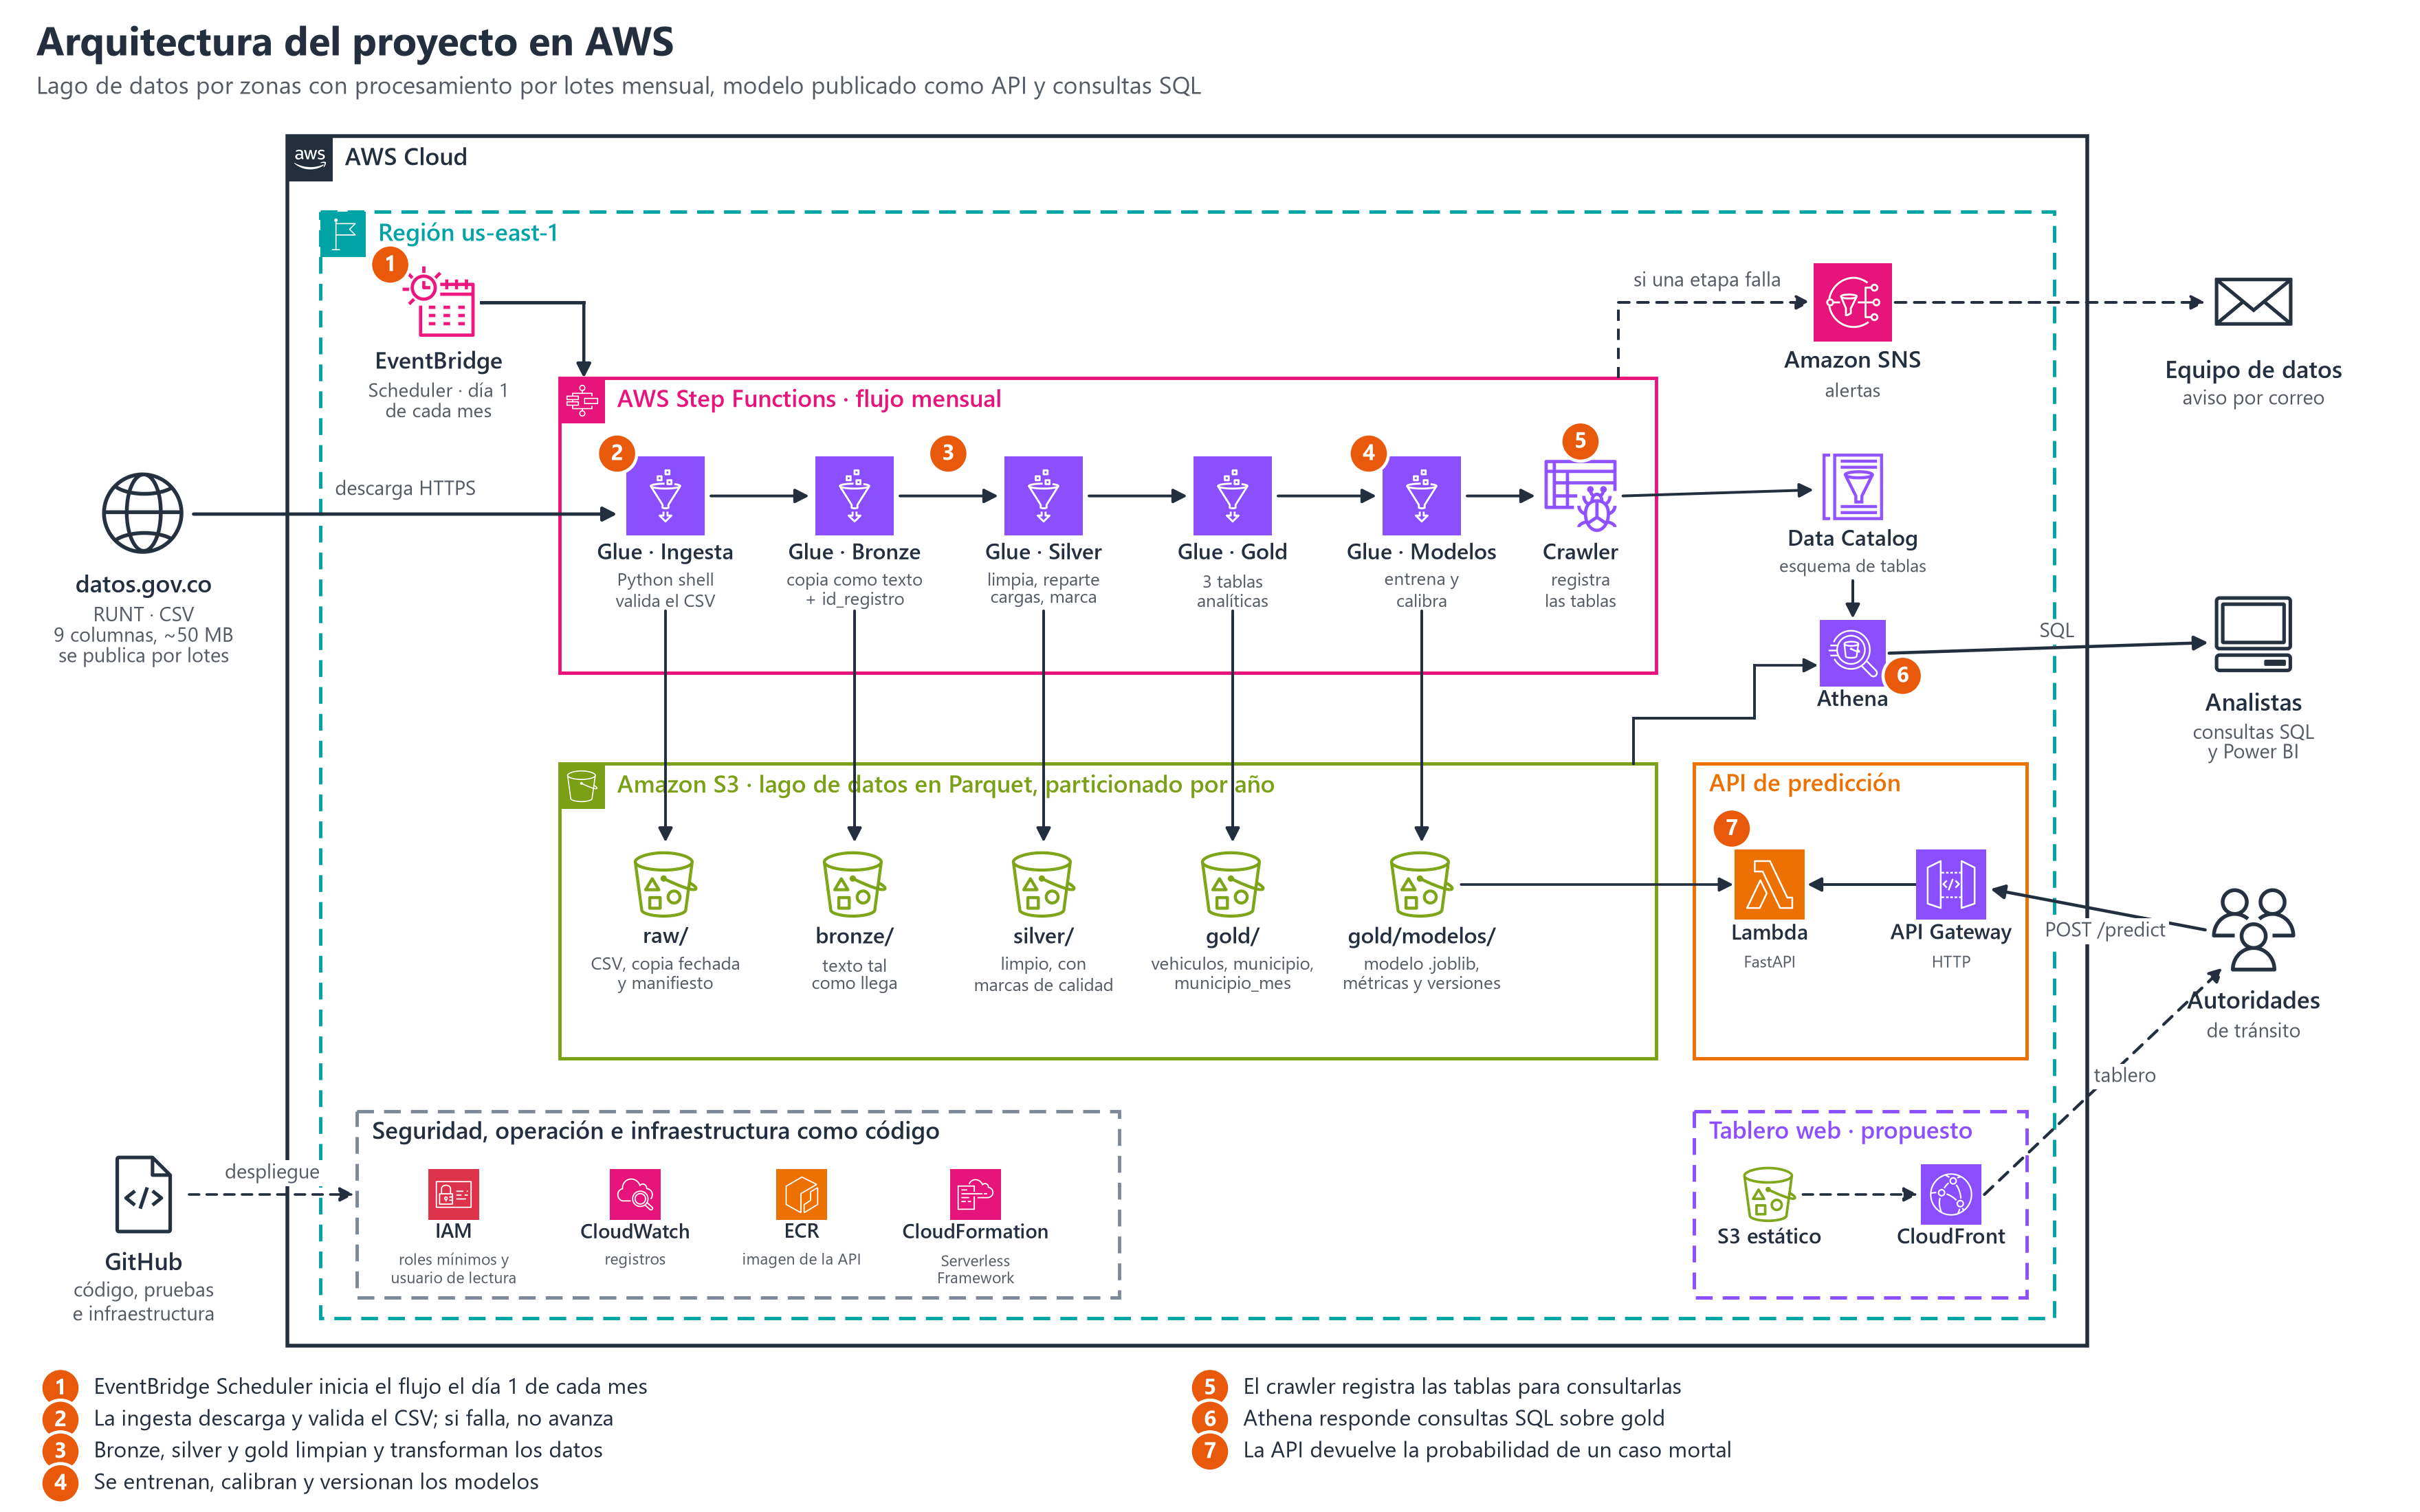
\includegraphics[width=\linewidth,height=0.9\textheight,keepaspectratio]{arquitectura_aws}
  \captionof{figure}{Arquitectura del proyecto en AWS, con los íconos oficiales de AWS (Amazon Web Services, 2026). Las líneas punteadas son alertas, despliegue o componentes propuestos para un escenario real.}\label{fig:arquitectura}
\end{landscape}}

\subsection{Desarrollo del proyecto}

El mismo código corre en un computador personal y en AWS. Todo acceso a datos pasa por un módulo de configuración: si la variable \texttt{DATA\_DIR} apunta a la carpeta local, lee y escribe ahí; si apunta a un bucket de S3, usa S3. Así probamos todo en local antes de desplegar.

Usamos Python con pandas, numpy, pyarrow, scikit-learn (Pedregosa et al., 2011) y joblib, porque son las librerías que AWS Glue trae disponibles. El flujo completo corre en unos siete minutos. Las semillas están fijas para que los resultados se repitan, y cada etapa se puede correr por separado. El código, las pruebas, las instrucciones y la infraestructura están en GitHub.

\subsection{Fuentes de datos y su naturaleza}

La fuente es un archivo de datos abiertos del portal datos.gov.co: estructurado, en CSV, de unos 50 MB, que se publica por lotes. No es transaccional ni llega en tiempo real. No trae datos personales y tiene licencia Creative Commons Atribución-CompartirIgual 4.0, así que citamos al Ministerio de Transporte y al RUNT y compartimos los datos derivados con la misma licencia.


\subsection{Ingesta}

La ingesta es por lotes y está automatizada. Un trabajo de AWS Glue de tipo Python shell descarga el CSV del portal y lo valida antes de dejarlo seguir: revisa que estén las nueve columnas, que la fecha tenga formato mes y año, que la gravedad solo tome sus dos valores, y que el número de filas y de vacíos sea razonable. Si todo está bien, guarda la copia vigente, una copia fechada en un histórico y una bitácora con la huella del archivo y el resultado de cada validación. Si algo falla, el archivo va a una carpeta de rechazados y la copia vigente no cambia. Si el portal no responde, usa una copia de respaldo.

Elegimos lotes porque así publica la fuente. Revisar el portal una vez al mes basta para recoger cada versión nueva.

\subsection{Almacenamiento}

\begin{itemize}
  \item \textit{Lago de datos.} Un bucket de S3 con una carpeta por zona. Silver y gold se guardan en Parquet, un formato por columnas que comprime bien y deja leer solo las columnas necesarias, particionado por año, que es el filtro más común en las consultas. El bucket está cifrado, bloquea el acceso público y borra solo los archivos temporales.
  \item \textit{Catálogo y motor SQL.} Un crawler de Glue registra las tablas de silver y gold en el Glue Data Catalog, y Amazon Athena las consulta con SQL sin servidores que administrar. Elegimos un motor SQL porque los datos son tablas y las consultas son analíticas: sumar, filtrar y agrupar. No hay escrituras frecuentes ni búsquedas por clave, que es donde una base transaccional o NoSQL tendría ventaja. Cada consulta tiene un límite de 1 GB leído para controlar el costo.
  \item \textit{Archivos.} El modelo entrenado se guarda como archivo joblib junto con un archivo de métricas que describe el entrenamiento, las variables y el umbral. Cada versión del modelo se registra en una carpeta propia, y la API puede servir una versión fija.
\end{itemize}

Gold tiene tres tablas principales: una fila por vehículo para el modelo, una fila por municipio y mes con conteos y alertas de cobertura para el tablero, y una fila por municipio para el agrupamiento. La etapa de modelos agrega las métricas, las predicciones, los grupos y la letalidad esperada.

\subsection{Ambiente de procesamiento}

Cada etapa, bronze, silver, gold y modelos, es un trabajo de AWS Glue 5.0 con dos trabajadores. AWS Step Functions las corre en orden, reintenta una vez la etapa que falle y avisa por correo con Amazon SNS. Al final corre el crawler para actualizar el catálogo. Amazon EventBridge Scheduler puede lanzar el flujo el día 1 de cada mes; se crea apagado para que un despliegue nunca inicie corridas por su cuenta.

Hoy cada etapa procesa los datos con pandas dentro del trabajo de Glue. Con 450 mil filas los datos caben en memoria y la corrida completa tarda minutos, así que un procesamiento distribuido no aportaría velocidad. Sabemos que la rúbrica pide un framework distribuido como Spark, y que pandas no reparte el trabajo entre nodos. El camino para crecer está preparado: los trabajos ya corren en el entorno Spark de Glue, y las transformaciones de silver y gold son operaciones de tablas que se traducen directamente a PySpark si el volumen aumenta, por ejemplo al sumar más fuentes o más años. Una versión anterior del proyecto, sobre los datos de Envigado, ya tenía estas etapas en Spark.

\subsection{Aplicaciones}

\textit{API de predicción.} El modelo se publica con FastAPI. Quien llama envía datos naturales, como el tipo, la marca, el año del modelo, la fecha, el departamento y la autoridad, y la API calcula las demás variables con las mismas funciones de la capa silver. Devuelve la probabilidad calibrada, si supera el umbral de alerta y la versión del modelo que respondió. Acepta lotes de hasta 100 vehículos y una llave de acceso opcional. En AWS corre en Lambda, a partir de una imagen guardada en Amazon ECR, detrás de un API Gateway HTTP. Tiene pruebas automáticas que la llaman con casos reales.

\textit{Consultas.} Athena responde consultas SQL sobre gold, y un usuario de solo lectura permite conectar Power BI.

\textit{Tablero.} Un tablero web que lee las tablas de gold, descrito en la sección~\ref{sec:visualizacion}.

\subsection{Despliegue en un escenario real}

Toda la infraestructura está escrita como código con Serverless Framework, que la traduce a AWS CloudFormation. Un comando la crea, otro corre el flujo y espera a que termine, y otro la borra por completo. El comando que corre el flujo termina con error si alguna etapa falla, así que sirve como prueba de extremo a extremo.

En una implementación real con una autoridad de tránsito haríamos estos cambios:

\begin{itemize}
  \item Encender la ejecución mensual y la alerta por correo.
  \item Publicar el tablero en S3 con CloudFront, para que se abra desde cualquier navegador con un enlace.
  \item Recalibrar el modelo cada vez que cambie la cobertura del registro, y revisar sus métricas antes de publicar una versión nueva.
  \item Guardar la llave de la API en un gestor de secretos y agregar alarmas de CloudWatch sobre errores y tiempos de respuesta.
\end{itemize}

\textit{Seguridad.} Cada servicio tiene su propio rol con los permisos mínimos que necesita. El usuario de Power BI solo puede consultar gold. Las credenciales viven en un archivo local que no se sube al repositorio.

\textit{Costos.} Con la infraestructura montada y sin correr, el costo es casi cero: Glue, Step Functions, el crawler, Athena y Lambda solo cobran cuando se usan, y el bucket guarda unos cientos de megabytes. Cada corrida usa cuatro trabajos de Glue pequeños y uno de Python shell.

% ------------------------------------------------------------------ 5
\section{Visualización y comunicación de datos}\label{sec:visualizacion}

\subsection{Requerimientos}

El tablero está pensado para las secretarías de movilidad, la Agencia Nacional de Seguridad Vial y la policía de tránsito. Son personas que deciden dónde poner controles y campañas, no analistas de datos. A partir de esto definimos seis preguntas que el tablero debe responder, una por página:

\begin{enumerate}
  \item ¿A dónde enviamos los controles y a qué vehículos?
  \item ¿Qué vehículos y departamentos concentran el riesgo?
  \item ¿Podemos confiar en los datos?
  \item ¿Qué hicimos para corregirlos?
  \item ¿Qué tan bien funciona el modelo y qué agrega?
  \item ¿Qué hacemos con esto?
\end{enumerate}

También pusimos requisitos prácticos: que se abra sin internet y sin instalar nada, que se actualice cuando corra el flujo, y que se pueda mostrar en Streamlit para la entrega.

\subsection{Análisis}

Siguiendo a Munzner (2014), revisamos qué datos se muestran, para qué tarea y cómo:

\begin{itemize}
  \item \textit{Datos.} Proporciones y conteos por categorías, como tipo de vehículo, edad y departamento; series por mes; y métricas del modelo.
  \item \textit{Tareas.} Ubicar dónde están los casos, comparar la letalidad entre grupos, encontrar anomalías en el reporte y entender qué tanto mejora el modelo frente a no tener modelo.
  \item \textit{Codificación.} Barras ordenadas para comparar, porque la longitud es lo que mejor se lee; un mapa por departamento para ubicar; barras por mes para ver la caída y la carga masiva; y cifras grandes para los mensajes clave.
\end{itemize}

\subsection{Diseño}

\begin{itemize}
  \item \textit{Una historia en orden.} Las páginas siguen el orden de la exposición: hallazgos, calidad del dato, tratamiento, modelo y acciones. Cada página responde una sola pregunta.
  \item \textit{Títulos que cuentan el hallazgo.} En lugar de «Letalidad por departamento», el título dice «Qué vehículos y departamentos concentran el riesgo».
  \item \textit{Color con propósito.} Una paleta de vía, amarillo y gris, poco saturada. El gris es el fondo de la comparación y el amarillo marca lo que hay que mirar, como el tractocamión o la barra del modelo ganador. Las barras llevan una línea con el promedio para que cada valor se lea frente a una referencia.
  \item \textit{Lenguaje sencillo.} Hablamos de «letalidad» y de «casos mortales hallados», no de prevalencia ni de sensibilidad, y explicamos cada métrica con una frase.
  \item \textit{Menos es más.} Quitamos gráficas que el equipo no lograba leer de un vistazo, como una gráfica de pesas y varias líneas cruzadas, y las cambiamos por barras.
\end{itemize}

\subsection{Implementación}

El tablero es una página web estática hecha con HTML, CSS y JavaScript, sin librerías externas. Las gráficas se dibujan en SVG desde el código. Un script lee las tablas de gold y genera el archivo de datos del tablero, así que cada vez que corre el flujo basta con volver a exportar. Para la entrega lo mostramos además dentro de Streamlit, que incrusta la misma página.

La interacción incluye filtros por periodo, departamento y tipo de vehículo en una sola barra superior; un mapa que cambia entre casos mortales y letalidad; información emergente con el detalle de cada dato; y navegación por páginas con el menú, los puntos del paginador o las flechas del teclado. La figura~\ref{fig:hallazgos} muestra la primera página.

\figura{fig_hallazgos}{1}{Página 1 del tablero: mapa de casos mortales por departamento y cifras clave.\label{fig:hallazgos}}

\figura{fig_acciones}{0.9}{Página 6 del tablero: acciones que se proponen a las autoridades de tránsito.\label{fig:acciones}}

\subsection{Validación}

Validamos el tablero de tres formas:

\begin{itemize}
  \item \textit{Las cifras.} Cada número sale de las tablas de gold, y comparamos los totales del tablero con los del CSV original y con los de las tablas que consulta Athena.
  \item \textit{La lectura.} En varias rondas de revisión del equipo marcamos lo que no se entendía y lo cambiamos: etiquetas que se montaban sobre las barras, gráficas de líneas difíciles de leer, barras muy separadas y textos técnicos.
  \item \textit{El funcionamiento.} Probamos que la página se abra sin internet con doble clic, dentro de Streamlit y en distintos tamaños de pantalla.
\end{itemize}

Queda pendiente una prueba de uso con personas de una secretaría de movilidad, resolviendo tareas concretas como encontrar los municipios con más letalidad de la esperada.

% ------------------------------------------------------------------ 6
\section{Conclusiones generales}

\begin{enumerate}
  \item \textit{Los vehículos de carga y las carreteras concentran la letalidad.} El tractocamión llega a 28,7~\%, cinco veces el promedio, y los registros de la policía de carreteras tienen siete veces la letalidad de los urbanos. Las motos, por volumen, aportan más de la mitad de los casos mortales.
  \item \textit{El modelo es útil para priorizar, con un aporte moderado.} Revisando el 15~\% de los registros encuentra el 61~\% de los casos mortales, cuatro veces más que el azar. Una regla simple ya captura buena parte de ese valor; el modelo agrega orden y probabilidades calibradas.
  \item \textit{El vehículo explica poco.} La autoridad que registra y el departamento pesan más que la marca o la edad. Para mejorar de verdad hacen falta variables que el registro no trae, como el tipo de vía, la hora y las víctimas.
  \item \textit{La calidad del registro es el hallazgo más urgente.} Medellín y Bogotá casi dejaron de reportar en 2025, hubo cargas masivas de reportes atrasados y cada secretaría reporta distinto. Sin tratarlo, la letalidad nacional parecía subir sin que el riesgo cambiara.
  \item \textit{Corregir antes de modelar cambió los resultados.} Recalcular la edad, repartir las cargas masivas y dejar fuera los meses anómalos evitó que el modelo aprendiera errores del reporte.
  \item \textit{La arquitectura es reproducible y barata.} El lago por zonas en S3, los trabajos de Glue orquestados con Step Functions, Athena y la API en Lambda se crean y se borran con un comando, y casi no cuestan cuando no corren. El paso pendiente es llevar las transformaciones a Spark si el volumen crece.
  \item \textit{Recomendación para las autoridades.} Priorizar controles a vehículos de carga en corredores viales, mantener las campañas para motociclistas, exigir al RUNT un reporte completo y a tiempo, y revisar primero los municipios cuya letalidad se aleja de lo esperado, como Soacha o Medellín.
\end{enumerate}

% ------------------------------------------------------------------ referencias
\section*{Referencias}
\addcontentsline{toc}{section}{Referencias}
\begin{list}{}{\leftmargin=1.2em \itemindent=-1.2em \itemsep=0.35em \parsep=0pt}
\small
\item Agencia Nacional de Seguridad Vial. (2025). \textit{Cifras preliminares del Observatorio Nacional de Seguridad Vial, enero-abril de 2025}. El Tiempo. \url{https://www.eltiempo.com/mas-contenido/se-han-reducido-las-victimas-fatales-por-siniestros-viales-en-2025-ansv-3455307}
\item Amazon Web Services. (2026). \textit{AWS Architecture Icons}, versión de julio de 2026. \url{https://aws.amazon.com/architecture/icons/}
\item Armbrust, M., Ghodsi, A., Xin, R., y Zaharia, M. (2021). Lakehouse: A new generation of open platforms that unify data warehousing and advanced analytics. En \textit{Conference on Innovative Data Systems Research (CIDR)}.
\item Breiman, L. (2001). Random forests. \textit{Machine Learning, 45}(1), 5-32. \url{https://doi.org/10.1023/A:1010933404324}
\item Chapman, P., Clinton, J., Kerber, R., Khabaza, T., Reinartz, T., Shearer, C., y Wirth, R. (2000). \textit{CRISP-DM 1.0: Step-by-step data mining guide}. SPSS.
\item Chen, T., y Guestrin, C. (2016). XGBoost: A scalable tree boosting system. En \textit{Proceedings of the 22nd ACM SIGKDD International Conference on Knowledge Discovery and Data Mining} (pp. 785-794). \url{https://doi.org/10.1145/2939672.2939785}
\item Congreso de la República de Colombia. (2022). \textit{Ley 2251 de 2022}, por la cual se dictan normas para el diseño e implementación de la política de seguridad vial con enfoque de sistema seguro. Diario Oficial 52.095. \url{http://www.secretariasenado.gov.co/senado/basedoc/ley_2251_2022.html}
\item Elkan, C. (2001). The foundations of cost-sensitive learning. En \textit{Proceedings of the 17th International Joint Conference on Artificial Intelligence} (pp. 973-978).
\item Friedman, J. H. (2001). Greedy function approximation: A gradient boosting machine. \textit{The Annals of Statistics, 29}(5), 1189-1232. \url{https://doi.org/10.1214/aos/1013203451}
\item Geurts, P., Ernst, D., y Wehenkel, L. (2006). Extremely randomized trees. \textit{Machine Learning, 63}(1), 3-42. \url{https://doi.org/10.1007/s10994-006-6226-1}
\item He, H., y Garcia, E. A. (2009). Learning from imbalanced data. \textit{IEEE Transactions on Knowledge and Data Engineering, 21}(9), 1263-1284.
\item Ke, G., Meng, Q., Finley, T., Wang, T., Chen, W., Ma, W., Ye, Q., y Liu, T.-Y. (2017). LightGBM: A highly efficient gradient boosting decision tree. \textit{Advances in Neural Information Processing Systems, 30}.
\item Knaflic, C. N. (2015). \textit{Storytelling with data: A data visualization guide for business professionals}. Wiley.
\item MacQueen, J. (1967). Some methods for classification and analysis of multivariate observations. En \textit{Proceedings of the Fifth Berkeley Symposium on Mathematical Statistics and Probability} (Vol. 1, pp. 281-297). University of California Press.
\item Mannering, F. L., y Bhat, C. R. (2014). Analytic methods in accident research: Methodological frontier and future directions. \textit{Analytic Methods in Accident Research, 1}, 1-22. \url{https://doi.org/10.1016/j.amar.2013.09.001}
\item Ministerio de Transporte. (2022). \textit{Decreto 1430 de 2022}, por medio del cual se aprueba el Plan Nacional de Seguridad Vial 2022-2031. \url{https://www.funcionpublica.gov.co/eva/gestornormativo/norma.php?i=191348}
\item Ministerio de Transporte. (2026). \textit{Vehículos involucrados en un accidente de tránsito Ley 2251-2022} [Conjunto de datos, fuente RUNT]. datos.gov.co. \url{https://www.datos.gov.co/d/6jmc-vaxk}
\item Munzner, T. (2014). \textit{Visualization analysis and design}. CRC Press.
\item Organización Mundial de la Salud. (2023). \textit{Global status report on road safety 2023}. OMS.
\item Pedregosa, F., Varoquaux, G., Gramfort, A., Michel, V., Thirion, B., Grisel, O., et al. (2011). Scikit-learn: Machine learning in Python. \textit{Journal of Machine Learning Research, 12}, 2825-2830.
\item Rousseeuw, P. J. (1987). Silhouettes: A graphical aid to the interpretation and validation of cluster analysis. \textit{Journal of Computational and Applied Mathematics, 20}, 53-65.
\item Saito, T., y Rehmsmeier, M. (2015). The precision-recall plot is more informative than the ROC plot when evaluating binary classifiers on imbalanced datasets. \textit{PLoS ONE, 10}(3), e0118432.
\item Savolainen, P. T., Mannering, F. L., Lord, D., y Quddus, M. A. (2011). The statistical analysis of highway crash-injury severities: A review and assessment of methodological alternatives. \textit{Accident Analysis \& Prevention, 43}(5), 1666-1676.
\item Vargas, J. (2025, 11 de marzo). En el 2024 murieron 8.271 personas por accidentes de tránsito, según la Agencia Nacional de Seguridad Vial. \textit{Xataka Colombia}. \url{https://www.xataka.com.co/vehiculos/2024-murieron-8-271-personas-accidentes-transito-agencia-nacional-seguridad-vial}
\item Zadrozny, B., y Elkan, C. (2002). Transforming classifier scores into accurate multiclass probability estimates. En \textit{Proceedings of the 8th ACM SIGKDD International Conference on Knowledge Discovery and Data Mining} (pp. 694-699).
\end{list}

\end{document}
